%% This is file `IPPbeamer.tex' version 2.2 (2022/07/23),
%% it is part of the IPP-bundle
%% Beamer-slides and tcolorbox-posters for IPP
%% ----------------------------------------------------------------------------
%%
%%  Copyright (C) 2020–2023 by Marei Peischl <marei@peitex.de>
%%
%% ============================================================================
%% This work may be distributed and/or modified under the
%% conditions of the LaTeX Project Public License, either version 1.3c
%% of this license or (at your option) any later version.
%% The latest version of this license is in
%% http://www.latex-project.org/lppl.txt
%% and version 1.3c or later is part of all distributions of LaTeX
%% version 2008/05/04 or later.
%%
%% This work has the LPPL maintenance status `maintained'.
%%
%% Thecurrent maintainer of this work is
%%   Marei Peischl <marei@peitex.de>
%%
%% ============================================================================
%%
\documentclass[
	english,% main language as global option
	logo=false,% logo to be used in the headline. Pre-defined values are: asdex, w7x, false. Initial value is empty
	eurofusion=false, %initial value is false
	titlegraphic=true, %initial value is false
	]{ippbeamer}

\usepackage{amsmath}
\usepackage{amsfonts}
\usepackage{amssymb}
\usepackage{amsthm}
\usepackage{bm}
\usepackage{caption}
\usepackage{xcolor}
\usepackage{csquotes}
\usepackage{enumerate}
\usepackage{faktor}
\usepackage{graphicx}
\usepackage{hyperref}
\usepackage{listings}
\usepackage{mathrsfs}
\usepackage{mathtools}
\usepackage{pgf,tikz}
\usepackage{pgfplots, pgfplotstable}
% \usepackage{showlabels}
\usepackage{svg}
\usepackage{tikz-cd}
\usepackage{url}

\usepackage{subcaption} 

\pgfplotsset{compat=1.18}
\usetikzlibrary{arrows}
\usetikzlibrary{decorations.pathreplacing,decorations.markings}

\definecolor{codegreen}{rgb}{0,0.6,0}
\definecolor{codegray}{rgb}{0.5,0.5,0.5}
\definecolor{codepurple}{rgb}{0.58,0,0.82}
\definecolor{backcolour}{rgb}{0.95,0.95,0.92}


\lstdefinestyle{mystyle}{
    backgroundcolor=\color{backcolour},   
    commentstyle=\color{codegreen},
    keywordstyle=\color{magenta},
    numberstyle=\tiny\color{codegray},
    stringstyle=\color{codepurple},
    basicstyle=\ttfamily\footnotesize,
    breakatwhitespace=false,         
    breaklines=true,                 
    captionpos=b,                    
    keepspaces=true,                 
    % numbers=left,                    
    numbersep=5pt,                  
    showspaces=false,                
    showstringspaces=false,
    showtabs=false,                  
    tabsize=2
}

\lstset{style=mystyle}

\captionsetup[figure]{labelformat=empty}

% \newtheorem{lemma}{Lemma}[section]
% \numberwithin{lemma}{section}
% \newtheorem{corollary}[lemma]{Corollary}
% \newtheorem{proposition}[lemma]{Proposition}
% \newtheorem{theorem}[lemma]{Theorem}

% \theoremstyle{definition}
% \newtheorem{assumption}[lemma]{Assumption}
% \newtheorem{definition}[lemma]{Definition}
% \newtheorem{example}[lemma]{Example}
% \newtheorem{remark}[lemma]{Remark}
% \newtheorem{problem}[lemma]{Problem}

\DeclareMathOperator{\curl}{curl}
\DeclareMathOperator{\diver}{div}

\newtheorem{assumption}{Assumption}




% some adjustments which are generally not available
\let\code\texttt
\let\file\texttt

% extended graphicspath to use separate image directories without the bundle being installed
\graphicspath{{}{img/}{img/titlegraphic/}}

\title{Solving the Quasi-Neutrality Equation on Surfaces}
% \subtitle{presentations using \LaTeX}
\author{Alexander Hoffmann, Martin Campos Pinto, Florian Hindenlang, Omar Maj, 
		Eric Sonnendrücker}
% \institute{\inst{1}pei\TeX{} \and\inst{2}Institut 2}
\date{\today}
% Additional Logo to be placed in the footer
% \logo{\includegraphics[height=\height]{example-image}}

\begin{document}


\frame{\titlepage}



\begin{frame}{Structure of multi-patch}

\begin{figure}[!h]
\begin{subfigure}{0.8\textwidth}
\centering
\tiny
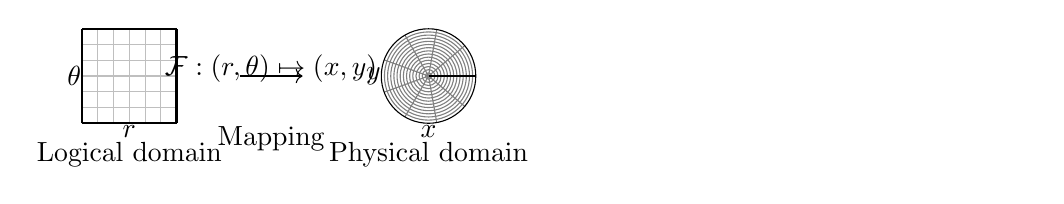
\begin{tikzpicture}[xscale = 0.4, yscale = 0.4]
	% logical grid
	\draw[lightgray] (0,0) grid [step = 0.5] (3,3);
	\draw[thick] (0,0) grid [step = 3] (3,3);
	
	\node at (-0.25, 1.5) {$\theta$}; 
	\node at (1.5, -0.25) {$r$}; 
	
	\node at (1.5,-1) {Logical domain} ; % subtitle
	
	% mapping
	\begin{scope}[xshift =1.5cm]	
		\draw[->] (3.5, 1.5) -- (5.5, 1.5); 
		\node at (4.5,1.75) {$\mathcal{F}:(r,\theta)\mapsto(x,y)$}; 
		
		\node at (4.5,-0.5) {Mapping} ; % title
	\end{scope}
	
	\begin{scope}[xshift = 11cm, yshift = 1.5cm]	
		% physical grid
		\def\Rmax{1.5}
		\foreach \r in {0, 0.1, ...,\Rmax} {
		    \draw[gray] (0,0) circle (\r);
		}
		\foreach \theta in {0, 40,...,360} {
    			\draw[gray] (0,0) -- (\theta:\Rmax);
		}
		
		\draw[black] (0,0) circle (\Rmax);
		\draw[black] (0,0) -- (0:\Rmax);
		
		\node at (-1.75, 0) {$y$}; 
		\node at (0, -1.75) {$x$}; 
		
		\node at (0,-2.5) {Physical domain} ; % subtitle
	\end{scope}
	
	\node at (30,0) { }; % just to put the figure on the left side on the slide. 
	
	
	
\end{tikzpicture}
\end{subfigure}
\begin{subfigure}{0.2\textwidth}
\centering
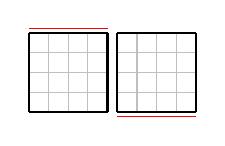
\begin{tikzpicture}[xscale = 0.5, yscale = 0.5]
	\draw[lightgray] (0,0) grid [step = 0.5] (2,2);
	\draw[thick] (0,0) grid [step = 2] (2,2);
	
	\draw[red] (0,2.125) -- (2,2.125);
	
	\begin{scope}[shift={(2.25,0)}]
		\draw[lightgray] (0,0) grid [step = 0.5] (2,2);
		\draw[thick] (0,0) grid [step = 2] (2,2);
		
		\draw[red] (0,-0.125) -- (2,-0.125);
	\end{scope}
\end{tikzpicture}
\caption{\scriptsize Simple interface.}
\end{subfigure}
\begin{subfigure}{0.2\textwidth}
\centering
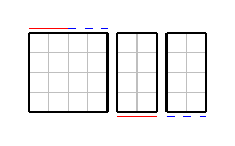
\begin{tikzpicture}[xscale = 0.5, yscale = 0.5]
	\draw[lightgray] (0,0) grid [step = 0.5] (2,2);
	\draw[thick] (0,0) grid [step = 2] (2,2);
	
	\draw[red] (0,2.125) -- (1,2.125);
	\draw[blue, dashed] (1,2.125) -- (2,2.125);
	
	\begin{scope}[shift={(2.25,0)}]
		\draw[lightgray] (0,0) grid [step = 0.5] (1,2);
		\draw[thick] (0,0) grid [xstep = 1, ystep=2] (1,2);
		\draw[red] (0,-0.125) -- (1,-0.125);
	\end{scope}
	
	\begin{scope}[shift={(3.5,0)}]
		\draw[lightgray] (0,0) grid [step = 0.5] (1,2);
		\draw[thick] (0,0) grid [xstep = 1, ystep=2] (1,2);
		\draw[blue, dashed] (0,-0.125) -- (1,-0.125);
	\end{scope}
	
\end{tikzpicture} 
\caption{\scriptsize T-joint. }
\end{subfigure}
\begin{subfigure}{0.4\textwidth}
\centering
\tiny
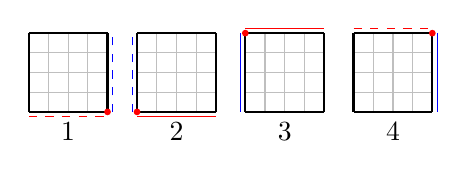
\begin{tikzpicture}[xscale = 0.5, yscale = 0.5]
	% grid
	\foreach \x in {0, ..., 3}{
		\begin{scope}[shift={(2.75*\x,0)}]
			\draw[lightgray] (0,0) grid [step = 0.5] (2,2);
			\draw[thick] (0,0) grid [step = 2] (2,2);
		\end{scope}
	}
	
	\node at (1,-0.5) {1};
	\node at (1+2.75,-0.5) {2};
	\node at (1+2.75*2,-0.5) {3};
	\node at (1+2.75*3,-0.5) {4};
	
	% Xpoint
	\draw[fill = red, color=red]  (2,0) circle (2pt);
	\draw[fill = red, color=red]  (2.75,0) circle (2pt);
	\draw[fill = red, color=red]  (2.75*2,2) circle (2pt);
	\draw[fill = red, color=red]  (2+2.75*3,2) circle (2pt);
	
	% Interfaces
	\draw[red] (0+2.75,-0.125) -- (2+2.75,-0.125);
	\draw[red] (0+2.75*2,2.125) -- (2+2.75*2,2.125);
	
	\draw[red, dashed] (0,-0.125) -- (2,-0.125);
	\draw[red, dashed] (0+2.75*3,2.125) -- (2+2.75*3,2.125);
	
	\draw[blue] (-0.125+2.75*2,0) -- (-0.125+2.75*2,2);
	\draw[blue] (2.125+2.75*3,0) -- (2.125+2.75*3,2);
	
	\draw[blue, dashed] (2.125,0) -- (2.125,2);
	\draw[blue, dashed] (-0.125+2.75,0) -- (-0.125+2.75,2);
	
	
\end{tikzpicture}
%\caption{X-point in logical domain.}
%\end{subfigure}
%\begin{subfigure}{0.2\textwidth}
	\includegraphics[width=3cm]{../images/X_point_in_physical.png}
\caption{\scriptsize X-point in logical and physical domain.}
\end{subfigure}
\caption{\footnotesize \label{Patches_logical_dom} Patches in the logical domain.}
\end{figure}


\end{frame}


%
%\begin{frame}{Decoupling into 2D problems in ideal situation}
%	Assume we have curvilinear coordinates $y^1, y^2, y^3$ s.t. 
%		for the basis vectors $\mathbf{e}_i = \partial \mathbf{x}/ \partial y^i$ we have
%		\begin{align*}
%			\mathbf{e}_1, \mathbf{e}_2 \perp \mathbf{b} \text{ and } \mathbf{e}_3 = \mu \mathbf{b}
%		\end{align*}		
%	
%	for some non-vanishing scalar field $\mu$.
%	Then the problem becomes w.r.t. these variables
%	\begin{align*}
%		-\frac{1}{\mu}\diver_{(1,2)} (\nu \mu \nabla_{(1,2)} \phi) &= \rho
%	\end{align*}
%	where $\diver_{(1,2)}$ is the divergence 
%	w.r.t. the first two variables
%	and analogous for $\nabla_{(1,2)}$. 
%\end{frame}
%\begin{frame}{Decoupling of the 2D problems in ideal situation}
%	\begin{exampleblock}{}
%		\textbf{IDEA:} Deal with the problem on the isosurfaces
%		of the third variable $y^3$ $\rightarrow$ the problems decouple	
%	\end{exampleblock}
%	
%
%	Assume for the 
%	surfaces $\{ y^3 = \text{const} \} \cap \partial \Omega \neq \varnothing$,
%	so Dirichlet boundary conditions can be imposed
%
%	\begin{alertblock}{Problem}
%		These surfaces do not exist for general vector fields
%	\end{alertblock}
%	\end{frame}
%
%
%
%\begin{frame}{Existence of orthogonal surfaces}
%	\begin{itemize}
%		\item Conditions for existence of these surfaces are given by the 
%			Frobenius theorem
%		\item There are multiple formulations of it. The most suited one for our purpose is:
%	\end{itemize}
%	\begin{exampleblock}{Frobenius Theorem (for codimension 1)}
%		Assume $\mathbf{B}$ is sufficiently regular and non-vanishing. Then the curvilinear coordinates as above 
%		exist, iff there are scalar fields $\alpha$ and $\beta$ s.t. $\mathbf{B} = \alpha \nabla \beta$. 
%	\end{exampleblock}
%
%	Another equivalent condition for the existence is
%	\begin{align*}
%		\mathbf{B}\cdot \curl \mathbf{B} = 0.
%	\end{align*}
%	\vspace*{-0.75cm}
%	\begin{exampleblock}{Question}
%		How large is $\mathbf{B}\cdot \curl \mathbf{B}$ in practice?
%	\end{exampleblock}
%
%\end{frame}
%
%\begin{frame}{Example: Nonexistence of orthogonal surfaces}
%	Counter-example from Omar Maj: \textbf{Cylindrically symmetric equilibrium}
%	\begin{align*}
%		\mathbf{B} = B_0 \mathbf{e}_z + \nabla \psi \times \mathbf{e}_z
%		= \begin{pmatrix}\partial_y \psi \\ -\partial_x  \psi \\ B_0 \end{pmatrix}
%	\end{align*}
%	with a constant $B_0 > 0$ and scalar function $\psi = \psi(x,y)$. 
%	We choose 
%	\begin{align*}
%		\psi(x,y) = \frac{a_0}{2} (x^2 + \kappa y^2).
%	\end{align*}
%	\begin{itemize}
%		\item Omar showed that this defines orthogonal surfaces iff 
%			$\kappa = -1$
%		\item For the imporant case $\kappa > 0$ (confined field
%			lines), orthogonal surfaces do not exist, not even locally.
%	\end{itemize}
%\end{frame}
%
%
%\begin{frame}{Surfaces given by the Dommaschk potential}
%	Let $\chi$ be the Dommaschk potential which is of the form
%	\footnote{W. Dommaschk (1986) - "Representations for vacuum potentials in stellarators", 
%				Computer Physics Communications 40}
%	\begin{align*}
%		\chi (R,\varphi, Z) = F_0 \varphi + \sum_{n,m} \chi_{n,m}(R, \varphi, Z), 
%			\quad \text{with }\Delta \chi_{n,m} = 0
%	\end{align*}
%	$\varphi$ is the toroidal angle and 
%	$F_0$ is a constant. 
%
%	\begin{alertblock}{}
%		If $\nabla \chi \approx \mathbf{B}$, 
%		we can take the isosurfaces of $\chi$. 	
%	\end{alertblock}
%
%\end{frame}
%	
%\begin{frame}{Angle between field from VMEC and Dommaschk potential}
%	\begin{itemize}
%		\item As a test, Florian Hindenlang took Dommaschk potential fitted to $\mathbf{B}$-field from VMEC for W7A 
%			with zero toroidal current and zero pressure
%			\footnote{Data provided by Nikita Nikulsin and Rohan Ramasamy, see Nikulsin et al (2022) - 
%			"JOREK3D: An extension of the JOREK nonlinear MHD code 
%			to stellarators"}.
%		\item Angle between $\mathbf{B}$ and $\nabla \chi$ less than $10^{-3}$
%	\end{itemize}
%
%	\begin{alertblock}{}
%		The equilibrium field $\mathbf{B}$ is almost orthogonal to the isosurfaces of $\chi$
%	\end{alertblock}
%
%	% The following plots are the angle 
%	% in degrees between 
%	% the magnetic field of W7A with zero toroidal current and zero pressure computed using 
%	% VMEC and the field 
%	% calculated from the Dommaschk potential 
%	% \footnote{Coefficients provided by Nikita Nikulsin and Rohan Ramasamy, see Nikulsin et al (2022) - 
%	% "JOREK3D: An extension of the JOREK nonlinear MHD code 
%	% to stellarators"}.
%	% Since the angle is almost zero, the magnetic field
%	% is almost orthogonal on the isosurfaces.
%
%
%	% \begin{columns}[
%	% 	onlytextwidth,%otherwise the whole pagewidth would be used
%	% 	c, %align vertically centered
%	% 	]
%	% \begin{column}{.5\linewidth}
%	% 		\includegraphics[width=\textwidth]{plots/Bfield_dommaschk_vs_gvec1.png}
%	% \end{column}
%	% \begin{column}{.5\linewidth}
%	% 		\includegraphics[width=\textwidth]{plots/Bfield_dommaschk_vs_gvec2.png}
%	% \end{column}
%
%\end{frame}
%
%\begin{frame}{Plot of angle between $\mathbf{B}$ and $\nabla \chi$}
%	Plots show the angle between $\mathbf{B}$ and $\nabla \chi$ in degrees on two poloidal cuts
%	\begin{figure}
%		\centering
%		\includegraphics[width=0.72\textwidth]{plots/Bfield_dommaschk_vs_gvec_2subplots.png}
%	\end{figure}
%
%\end{frame}
%
%\begin{frame}{Comparison with taking only $\varphi$ direction}
%	\begin{itemize}
%		\item Plots show the angle between $\mathbf{e}_\varphi$ and $\mathbf{B}$ on the same 
%				poloidal cuts
%		\item The angle is larger by 4 orders of magnitude in our example
%	\end{itemize}
%	\begin{figure}
%		\centering
%		\includegraphics[width=0.7\textwidth]{plots/B_vs_toroidal_direction.png}
%		\caption*{\footnotesize{Angle between $\mathbf{B}$ and 
%				  $\mathbf{e}_\varphi$ in degrees}}
%	\end{figure}
%\end{frame}
%
%
%\begin{frame}{Isosurfaces of the Dommaschk potential}
%	\begin{columns}[
%		onlytextwidth,%otherwise the whole pagewidth would be used
%		c, %align vertically centered
%		]
%	\begin{column}{.5\linewidth}
%			\includegraphics[width=\textwidth]{plots/compare_gvec_dommaschk.png}
%	\end{column}
%	\begin{column}{.5\linewidth}
%			\includegraphics[width=\textwidth]{plots/surfaces_with_magnetic_field_sideview.png}
%	\end{column}
%	\end{columns}
%
%	\begin{itemize}
%		\item Grey surfaces: Isosurfaces of the Dommaschk potential
%		\item Green surfaces: Isosurfaces of an approximate flux 
%			surface invariant computed from the Dommaschk potential
%		\item Dark blue glyphs: Magnetic field from VMEC
%	\end{itemize}
%\end{frame}
%
%\begin{frame}{Comparison on W7-X}
%	\includegraphics[width=\textwidth]{plots/compare_for_w7x_gvec_dommaschk_on_gvecdata_upper_plots.png}
%\end{frame}
%
%\begin{frame}{Comparison on W7-X}
%	\includegraphics[width=\textwidth]{plots/compare_for_w7x_gvec_dommaschk_on_gvecdata_lower_plots.png}
%\end{frame}
%
%
%\begin{frame}{Computing generalized potentials}
%	$\mathbf{B}$ defines orthogonal surfaces 
%	iff $\mathbf{B} = \alpha \nabla \beta$, but there exist no such $\alpha$ and $\beta$ in general.
%
%	\begin{exampleblock}{}
%		\textbf{Idea:} Approximate $\mathbf{B}$  with vector fields of the form $\alpha \nabla \beta$
%	\end{exampleblock}
%
%	Define the error functional 
%	\begin{align*}
%		J(\alpha, \beta) = \int_U \left| \mathbf{B} - \alpha \nabla \beta \right|^2 \, dx
%	\end{align*}
%	where $U \subseteq \Omega$ is a toroidal cut of the domain of interest
%	and solve the minimization problem
%	\begin{align*}
%		\min_{\alpha, \beta} J(\alpha, \beta)
%	\end{align*}
%
%\end{frame}
%
%
%\begin{frame}{Discrete optimization problem}
%	Use splines for the discretization, so the discrete minimization problem reads
%	\begin{align*}
%		\min_{\alpha_h, \beta_h \in V^0_h} J(\alpha_h, \beta_h)
%	\end{align*}
%	where $V^0_h$ is a pushforward tensor product spline space. 
%
%
%	\begin{alertblock}{}
%		Since we are interested in the surfaces only, these spline spaces can be chosen
%		local in the toroidal angle $\zeta \rightarrow$ Well suited for parallelization
%	\end{alertblock}
%
%	\begin{exampleblock}{}
%		Another discretization than splines is also possible.
%	\end{exampleblock}
%\end{frame}
%
%\begin{frame}{Gradient descent}
%	The Gateaux derivative of the functional is 
%	\begin{align*}
%		\delta_\alpha J(\alpha, \beta; \alpha_1) &= 
%			-2 \int_\Omega (\mathbf{B} - \alpha \nabla \beta) \cdot (\alpha_1 \nabla \beta) \, dx \text{ and } \\
%		\delta_\beta J(\alpha, \beta; \beta_1) &= 
%			-2 \int_\Omega (\mathbf{B} - \alpha \nabla \beta) \cdot (\alpha \nabla \beta_1) \, dx
%	\end{align*}
%
%	\begin{align*}
%		\alpha_h = \sum_{i=1}^{N} \mu_i \Lambda_i, \quad \beta_h = \sum_{i=1}^{N} \lambda_i \Lambda_i. 
%	\end{align*}
%	\begin{align*}
%		\frac{\partial}{\partial \bm{\mu}} J(\alpha_h, \beta_h)
%			&= \bigg( -2 \int_\Omega (\mathbf{B} - \alpha_h \nabla \beta_h) 
%			\cdot (\Lambda_i \nabla \beta_h) \bigg)_{i=1}^N \\
%		\frac{\partial}{\partial \bm{\lambda}} J(\alpha_h, \beta_h)
%			&= \bigg( -2 \int_\Omega (\mathbf{B} - \alpha \nabla \beta_h) 
%			\cdot (\alpha_h \nabla \Lambda_i)\bigg)_{i=1}^N
%	\end{align*}
%
%\end{frame}
%
%\begin{frame}[fragile]{Assembly of the gradients using Psydac library}
%	\begin{itemize}
%		\item Gradients are finite dimensional representations of 
%			linear forms $\rightarrow$ can be easily assembled using Psydac
%			\footnote{Güçlü, Y., Hadjout, S. and Ratnani, A. PSYDAC: a high-performance IGA library in Python. 2022.
%			(\url{https://github.com/pyccel/psydac})} 
%			
%		\item  Acceleration with Pyccel achieves speedup by a factor $\approx$1000
%			compared to Python
%	\end{itemize}
%	\begin{lstlisting}[language=Python]
%expr = -2*(alpha*dot(B, grad(beta1)) 
%           - alpha**2 * dot(grad(beta), grad(beta1)))
%lambda_deriv_symbolic = LinearForm(beta1, integral(domain, expr))
%lambda_deriv_discrete = discretize(lambda_deriv_symbolic, 
%                                   domain_h, 
%                                   derham_h.V0, 
%                                   backend=PSYDAC_BACKEND_GPYCCEL)
%lambda_deriv = lambda_deriv_discrete.assemble(B=B_h, 
%                                              alpha=alpha_h, 
%                                              beta=beta_h).toarray()	
%	\end{lstlisting}
%
%\end{frame}
%\begin{frame}{Gradient descent}
%	Using this the gradient and functional evaluation 
%	is feasible for gradient descent.
%
%	\begin{exampleblock}{Outlook}
%		So far, we have only run the algorithm for test examples where the field is 
%		given as a gradient. We want to try the following tests:
%		\begin{itemize}
%			\item Use a magnetic field from GVEC and use the Dommaschk potential 
%					as initial guess to see if we can improve the
%					approximation
%			\item Symmetric cylinder geometry from Omar's counterexample
%			\item Analytical Grad-Shafranov geometry
%		\end{itemize}
%	\end{exampleblock}
%\end{frame}
%
%
%\begin{frame}{Different approaches to finding the surfaces}
%	\textbf{Taking poloidal planes}
%	\begin{itemize}
%		\item Captures the dominant part of the field
%	\end{itemize}
%	\textbf{Isosurfaces of the Dommaschk potential}
%	\begin{itemize}
%		\item Good approximation for vacuum fields
%		\item Improvement by several orders of magnitude possible
%	\end{itemize}
%	\textbf{Generalized potentials}
%	\begin{itemize}
%		\item Most general approach
%		\item Not current free and thus possibly better for fields with strong current
%		\item Not tested on physically relevant fields yet
%	\end{itemize}
%	
%\end{frame}
%
%\begin{frame}{Solving the quasi-neutrality equation on the surfaces}
%	This material is taken from the Acta Numerica paper from Dziuk and Elliott
%	\footnote{Dziuk, Elliott (2013), "Finite Element Methods for Surface PDEs", 
%	Acta Numerica, pp. 289-396.}.
%	There are three main ideas: 
%	\begin{enumerate}
%		\item Use the potential to solve the PDE on all level sets simultaneously 
%				(implicit surface FEM)
%		\item Solve the PDE locally in a small neighborhood of a surface 
%				(Unfitted bulk FEM)
%		\item Discretize the surface directly (not discussed here)
%	\end{enumerate}
%\end{frame}
%
%
%
%\begin{frame}{Implicit surface FEM}
%	We want to solve the Poisson equation on level sets of $\beta$.
%	For a potential $\beta$, we get the normal field
%	\begin{align*}
%		\mathbf{n} \vcentcolon= \frac{\nabla \beta}{|\nabla \beta|}
%	\end{align*}
%	and define 
%	\vspace*{-0.25cm}
%	\begin{align*}
%		\nabla_\beta f \vcentcolon= P_\beta \nabla f, \quad P_\beta = I - \mathbf{n} \otimes \mathbf{n}.
%	\end{align*}
%	Then for a equation 
%	\vspace*{-0.25cm}
%	\begin{align*}
%		- \nabla \cdot (P_\beta \nabla \phi |\nabla \beta |) + c \phi |\nabla \beta | = 
%			f |\nabla \beta |
%	\end{align*}
%	with some scalar fields $f$ and $c$ with $c > \bar{c} > 0$, the weak formulation
%	reads
%	\begin{align*}
%		\int_\Omega \nabla_\beta \phi \cdot \nabla_\beta \eta |\nabla \beta | \, dx 
%			+ \int_\Omega c \phi \eta |\nabla \beta | \, dx 
%			= \int_\Omega f \eta |\nabla \beta | \, dx.
%	\end{align*}
%	where we implicitely used a no flux-boundary condition across 
%	$\partial \Omega$. 
%\end{frame}
%
%\begin{frame}{Implicit surface FEM}
%	This can be discretized on the domain $\Omega$ and we have existence,
%	uniqueness, convergence and regularity results.
%
%	\begin{exampleblock}{Outlook}
%		\begin{itemize}
%			\item In our case, the situation is slightly different due to Dirichlet boundary conditions
%			and $c = 0$
%			\item It is mostly standard elliptic theory for FE being used, 
%					which should be applicable
%			\item Instead of the full domain $\Omega$,
%					we can take subdomains $\Omega \cap \{ c_1 < \beta < c_2 \}$ for 
%					parallelization because the boundary conditions on the limiting surfaces
%					$\{ \beta = c_i \}$, $i=1,2$, vanish.
%		\end{itemize}
%	\end{exampleblock}
%\end{frame}
%
%\begin{frame}{Unfitted bulk FEM}
%	\small 
%	\begin{itemize}
%		\item Idea: Use already existing 3D mesh and discretize the 
%			problem only on the elements intersecting the surface (or a neighborhood of it)
%		\item Approach using implicit surfaces
%			is localized without the need to mesh the surface directly
%	\end{itemize}
%	\begin{figure}
%		\centering	
%		\includegraphics[width=0.7\textwidth]{unfitted_bulk_method_mesh.png}
%		% \caption{{\footnotesize Visualization of the area of computation of the unfitted bulk FEM for a curve.}}
%	\end{figure}
%\end{frame}
%
%\begin{frame}{Appendix: Derivation of the PDE in two variables}
%	Let 
%	\begin{align*}
%		\mathbf{b} = b^i \mathbf{e}_i
%	\end{align*}
%	so 
%	\begin{align*}
%		\nabla \phi \cdot \mathbf{b} = \frac{\partial \phi}{\partial x^i} b^i.
%	\end{align*}
%	and so 
%	\begin{align*}
%		\nabla_\perp \phi = \nabla \phi - (\mathbf{b} \cdot \nabla \phi) \mathbf{b}
%		= \bigg[ \frac{\partial \phi}{\partial x^i} g^{ij} 
%			- \bigg( \frac{\partial \phi}{\partial x^k} b^k \bigg) b^j \bigg] \mathbf{e}_j
%	\end{align*}
%	With the given assumptions $b^3 = 1/\mu$, $b^1 = b^2 = 0$, 
%	$g^{12} = g^{13} = 0$ and $g^{33} = 1/\mu^2$. This gives 
%	\begin{align*}
%		\nabla_\perp \phi = \sum_{i,j=1}^{2} g^{ij} \frac{\partial \phi}{\partial x^i}  \mathbf{e}_j
%			= \nabla_{(1,2)} \phi.
%	\end{align*}
%\end{frame}
%
%\begin{frame}{Appendix: Derivation of the PDE in two variables}
%	Let $G$ be the metric tensor and $\tilde{G}$ be the metric tensor of the first 
%	two coordinates, $g$ be the metric determinant and $\tilde{g}$ be the metric determinant
%	of the first two coordinates. Then we have $\sqrt{g} = \sqrt{\tilde{g}} \mu$ 
%	Taking the general divergence in curvilinear coordinates we have 
%	\begin{align*}
%		\frac{1}{\sqrt{g}}\sum_{i=1}^3 \frac{\partial (\sqrt{g} \nu (\nabla_\perp \phi)^i)}{\partial x^i}
%		= \frac{1}{\sqrt{\tilde{g}} \mu}\sum_{i=1}^{2} 
%			\frac{\partial (\sqrt{\tilde{g}} \mu \nu (\nabla \phi)^i)}{\partial x^i}
%		= \frac{1}{\mu} \diver_{(1,2)} (\nu \mu \nabla_{(1,2)} \phi)
%	\end{align*}
%\end{frame}
%
%\begin{frame}{Appendix: Proof that orthogonal surfaces exist only for $\kappa = -1$}
%	Let $\beta$ be the $1$-form corresponding to $\mathbf{B}$. Then a necessary condition for 
%	the surfaces to exist is 
%	\begin{align*}
%		\beta \wedge d\beta = 0.
%	\end{align*}
%	We have in our case
%	\begin{align*}
%		\beta = a_0 (\kappa y dx - x dy) + B_0 dz
%	\end{align*}
%	and then
%	\begin{align*}
%		\beta \wedge d\beta = - B_0 a_0 (\kappa+1) dx \wedge dy \wedge dz 
%	\end{align*}
%	and thus $\beta \wedge d\beta$ iff $\kappa = -1$.
%\end{frame}
%
%\begin{frame}{Appendix: Frobenius theorem (vector field formulation)}
%	There are two main formulations of the Frobenius theorem. The first one is
%	for vector fields on manifolds. Let $M$ be a manifold of class $C^p$, $p\geq 2$. 
%	We call a subbundle $E$ of the tangent bundle \textbf{locally integrable} at $x_0$ if 
%	for any $x_0 \in M$ there exist a submanifold $N$ s.t. 
%	$T_{x_0}N = E_{x_0}$. We call $E$ integrable if it is integrable everywhere.
%
%	\begin{alertblock}{Frobenius theorem (vector field formulation)}
%		Let $E$ be a subbundle 
%		of the tangent bundle. 
%		Then $E$ is integrable iff
%		for any two vector fields $X$, $Y$ with values in $E$ we have 
%		$[X,Y] \in E$ where $[\cdot,\cdot]$ is the Lie bracket.
%	\end{alertblock}
%\end{frame}
%
%\begin{frame}{Appendix: Frobenius theorem (differential forms formulation)}
%	\small
%	The general version of the one mentioned at the beginning is
%	\begin{alertblock}{\small Frobenius theorem (differential form formulation)}
%		Let $M$ be a smooth manifold.
%		If we have a Pfaffian system $\mathcal{I} = \{ \theta^1, ..., \theta^s, d\theta^1, ..., d\theta^s \}$
%		s.t. 
%		\begin{align*}
%			d\theta^\sigma \wedge \theta^1 \wedge \dots \wedge \theta^s = 0 
%				\quad \text{for }1\leq \sigma \leq s.
%		\end{align*}
%		Then for every $x \in M$, there exist local coordinates $y^1$, $y^2$, ..., $y^n$ 
%		s.t.
%		\begin{align*}
%			\mathcal{I} = \{ dy^1, dy^2, ..., dy^s \}.
%		\end{align*}
%		The other direction is trivially true.
%		Also, the local integral manifold is given by the level sets 
%		$\{ y^1 = c_1 , y^2 = c_2, ..., y^s = c_s \}$ for real constants 
%		$c_i$.
%	\end{alertblock}
%	This theorem can be globalized in the sense, that through every $x \in M$ passes a unique
%	maximal integral manifold $N$. It is maximal in the sense that every other integral manifold
%	going through $x$ is included in $N$.
%\end{frame}


\end{document}

